

\chapter{Discussion}
\label{chapter:discussion}

The previously presented evaluation classifies 7 different map visualizations that contain clusters (5 map types and 2 examples), as well as 9 cluster visualization techniques (2 glyphs, 3 pixel-based and 4 geometric / diagrams). Each visualization has been evaluated against a limited set criteria which are considered as important for showing clustered, multi-variate data on maps.

All visualizations, with the exception of the Wind history example, fulfill the primary criterion of \textbf{being able to indicate the number of items within clusters}. This makes sense, as in many cases \textit{seeing overlap density} is an important feature of the visualization to indicate the amount of overplotting and tell the user an estimate of what to expect within the cluster. In the case of the Wind history example this is not necessary because all clusters are of the same size and visualize their inner data ratio as part of the polar area chart. Given the many classifications of ``possibly'' and considering the presented examples, it seems like fulfilling this criterion heavily depends on the needs of the use case. The fact, that all evaluated visualization techniques support showing cluster sizes, apparently correlates with their selection process. Naturally, those visualization approaches have been evaluated that seemed logical for visualizing clustered data. 

On the contrary, few visualization techniques fulfill the criterion of \textbf{showing the cluster area}. The presented glyphs, pixel-based and diagram techniques do not have this feature as their shape is predefined. On the other hand, the Hull example indicates that a shape that indicates area can also be combined with an arbitrary shape inside.

While most cluster visualization techniques fail at indicating areas, they are perfectly suited for \textbf{showing extra cluster info}. Glyphs, geometric-techniques and diagrams appear suitable for visualizing cluster info of lower complexity while pixel-based techniques are geared towards multi-variate data of higher complexity.


Given the general discussion of the study results, a practical evaluation of Geocluster is added to the discussion.

\section{Geocluster visualization}
\label{chapter:geocluster-vis}

Geocluster\footnote{\url{http://drupal.org/project/geocluster}} is a server-side clustering implementation for mapping with Drupal based on Geohash. Refer to the complete thesis on Geocluster for an explanation of related concepts as Drupal, the Drupal mapping stack, Bounding Box strategies etc. \cite{geocluster-thesis}. Two visualizations for Geocluster have been implemented:

\begin{itemize}

\item \textbf{Geocluster default visualization}

A simple Geocluster visualization component has been built to support the display of clustered markers on interactive maps based on the output of the server-side clustering implementation. It extends the Bounding Box strategy of the Leaflet GeoJSON module in oder to create numbered markers that visualize the cluster sizes. Clicking on a clustered marker will zoom into the map in order to explore the data on a more granular level. Figure \ref{fig:map-clustered} demonstrates an example screenshot of the Geocluster visualization. Compare this with an unclustered map, containing the same amount of items in figure \ref{fig:map-unclustered}.


\hspace*{-1.5cm}\parbox [h]{0.5\textwidth}{
    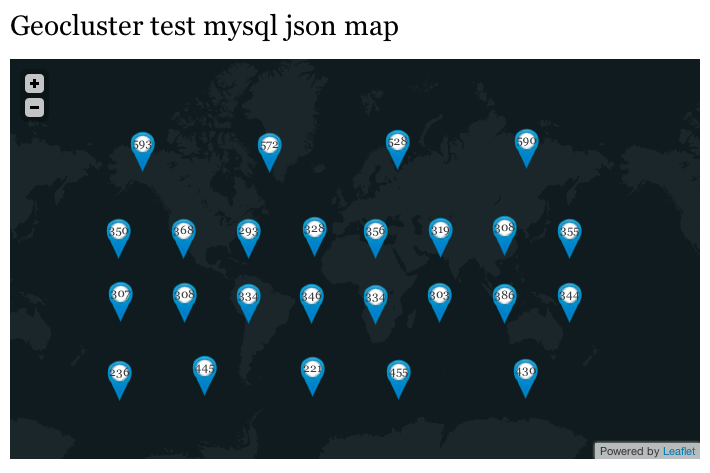
\includegraphics [width=\linewidth]{figures/map_clustered.png}
    \captionof {figure}{Geocluster visualization}
    \label{fig:map-clustered}
}
\hfill
\hspace{0.5cm}
\parbox [h]{0.5\textwidth }{
    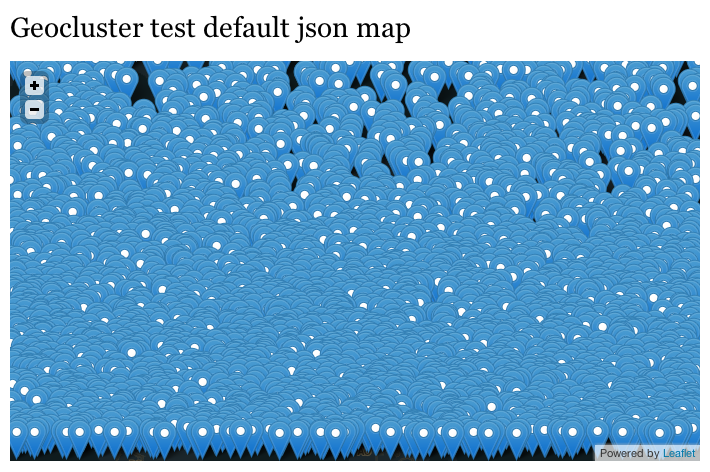
\includegraphics [width=\linewidth]{figures/map_unclustered.png}
    \captionof {figure}{Unclustered Leaflet map}
    \label{fig:map-unclustered}
}


The visualization component of Geocluster is based on a GeoJSON-feed provided by the server-side clustering implementation. It uses the JavaScript Bounding Box strategy to dynamically update results for the current viewport after zooming or panning the map. The cluster visualization is very simple and based on a code snippet for numbered markers on github\footnote{\url{https://gist.github.com/comp615/2288108}}.


\item \textbf{GeoRecruiter}

\begin{figure}[h]
  \begin{center}
    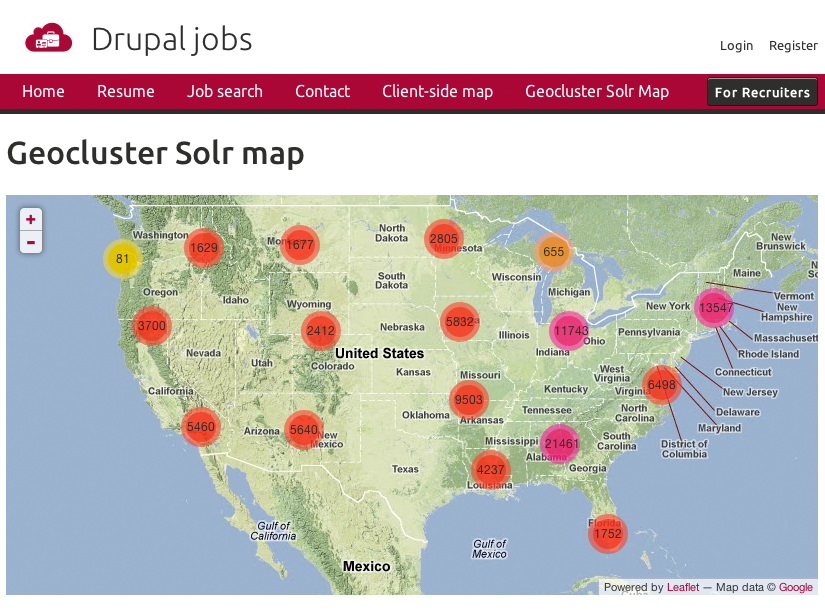
\includegraphics[width=1\textwidth]{figures/drupaljobs_geocluster_solr.png}
    \caption{Screenshot of map that visualized job search results on a map using Solr-based clustering on a Drupaljobs test installation.}
    \label{fig:drupaljobs-geocluster-solr}
  \end{center}
\end{figure}

A practical use case for server-side geo clustering has been implemented for the Recruiter job board solution. It supports spatial search capabilities of the Recruiter distribution by visualizing a large amount of job offers on e-recruitment websites. The prototype being discussed has been developed, based on a copy of the Drupaljobs website\footnote{\url{http://drupaljobs.epiqo.com}}.

\begin{quote}
\textit{Recruiter} is a Drupal distribution for building Drupal based e-recruitment platforms. Users can register either as recruiter and post job classifieds or they can register as applicants and fill out their resume. A faceted search helps users to find jobs and possible job candidates.\footnote{\url{http://drupal.org/project/recruiter}}. \textit{Drupaljobs} is provided as a show case for the Recruiter distribution. Its base features allow to create and search for job offers by companies as well as resumes of registered applicants on the e-recruitment platform.
\end{quote}


A map visualizes the clustered job search results. In order to enhance the representation of clusters and to experiment with interaction, the CSS styles of the client-side clustering library Leaflet.markercluster have been adapted and extended with additional colors for large clusters. A visualization of a map within the Drupaljobs test installation is provided in figure \ref{fig:drupaljobs-geocluster-solr}.




\end{itemize}

\section{Visual evaluation of Geocluster}

Two visualizations have been provided: first, the Client-side Geocluster Visualization component as visualized in figure \ref{fig:map-clustered} and second, an alternative visualization similar to the Leaflet.markercluster library for the GeoRecruiter use case, see figure \ref{fig:drupaljobs-geocluster-solr}.

Both implementations fulfill most of the clutter reduction criteria from chapter \ref{clutter-reduction}:

\begin{enumerate}

\item \textit{Overlap} is avoided by visualizing a non-overlapping clustering of points, as created by geohash-based clustering algorithm of Geocluster.

\item \textit{Spatial information} is expressed as an aggregate of latitude and longitude values for each cluster, approximating its centroid. One problem with the current implementations is, that clusters aren't ``stable''. In some experiments, changes to the bounding box will cause a change of cluster assignment. Intuitively, this leads to confusion of the user and should be investigated upon further. 

\item The Leaflet Bounding Box strategy implementation allows to \textit{localize} the view by panning and zooming and therefore reduce the display to a specific region.

\item \textit{Scalability} is provided by the underlying clustering algorithm, as evaluated in the publication on Geocluster \cite{geocluster-thesis}.

\item The configuration options of Geocluster allow to \textit{adjust} the minimum distance between clusters. Additional configuration options are provided by the Views integration of the Geocluster module. Still, the configuration options could be expanded for example to control visual parameters of clusters \cite{geocluster-thesis}.

\item The criterion of \textit{showing point/line attributes} is fulfilled only in a very limited way. Both implementations are currently restricted to displaying the number of items within a cluster as the only aggregate value. In order to support complex visualization techniques for multivariate data as discussed in chapter \ref{chapter:cluster-vis}, the clustering implementation needs to provide the required, aggregate values of the underlying data.

\item As explained in the discussion of the \textit{discriminating points/lines} criterion, its definition seems unclear. Clustered items and individual points are visualized in a different way, which can be seen as a fulfillment. On the other hand, the visualization currently doesn't provide any means of inspecting clusters. Only a list of identifiers of the items within a cluster is provided. Based upon the identifiers, a popup could be used to visualize the items a in more detailed way.

\item With regards to \textit{overlap density}, the number of items within clusters is indicated by both visualizations, but using different means. The Geocluster visualization doesn't make use of visual attributes like size or color, instead it creates a marker glyph that contains the number of items using textual representation. The GeoRecruiter prototype uses a color ramp that indicates low cluster densities from green and yellow to high densities indicated by tones of red and violet.

\end{enumerate}

\begin{figure}[h]
  \begin{center}
    \hspace*{-1.5cm}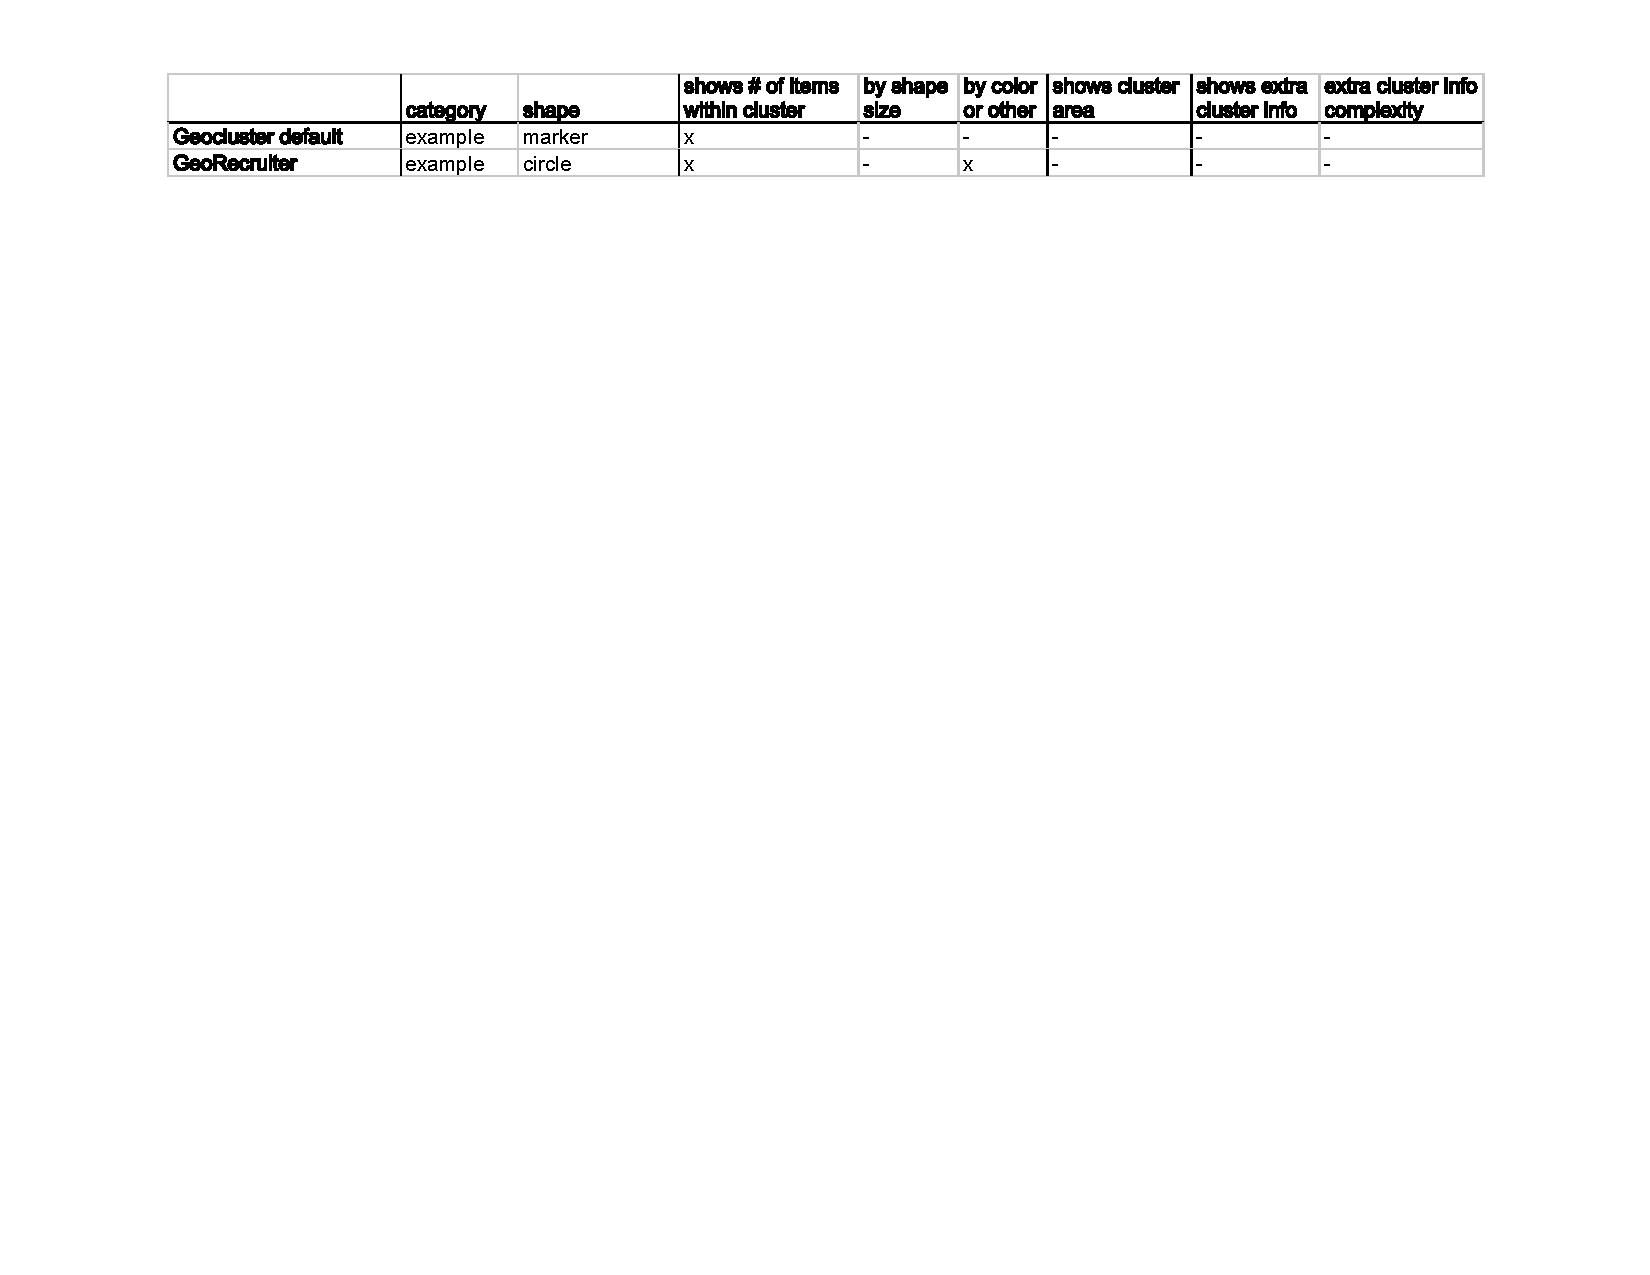
\includegraphics[width=1.2\textwidth]{figures/vis_eval_geocluster.pdf}
    \caption{Evaluation of Geocluster visualization techniques for clusters on a map. Legend:~`x':~yes,~`\textasciitilde': possibly, `-': no.}
    \label{fig:vis-eval-geocluster}
  \end{center}
\end{figure}

Next, the evaluation of visualization techniques for clusters on map presented in \ref{chapter:eval-vis} is applied to the two Geocluster implementations as illustrated in figure \ref{fig:vis-eval-geocluster}. It reiterates some key aspects identified by the previous discussion of clutter reduction criteria.

\textbf{Cluster sizes}: Both visualizations show the number of items within a cluster, but only the GeoRecruiter example uses color and none of them encodes the size of a cluster into the shape size. As naturally, a cluster with more items can be visualized larger than smaller clusters, the algorithm could be improved for growing clusters by their size. The bigger size of a cluster would therefore reduce the distance to its neighbor clusters, potentially merging additional neighbors into it. Andrew Betts describes a similar approach under the term \textit{``Grid based viral growth argorithm''}~\cite{web:clustering-google}.

\textbf{Cluster areas}: Neither implementation provides a visual indicator for showing cluster areas. Again, the server-side clustering implementation would need to provide this information. Instead, for performance reasons, only the number of items within clusters is provided as an aggregate value.

\textbf{Extra cluster info}: Similarly, no additional data about aggregates within clusters is exposed by the clustering implementation. This might suffice the use case of clustering points on maps for reducing clutter, but potentially hides a lot of information that could be displayed as part of the cluster visualization. 

On a note on performance of the interaction, for low zoom levels, the roundtrip to the server for fetching a separate clustered result on every bounding box change can be an overhead. Christopher Calid proposes a way of ``Progressively enhance server-side with client-side clustering''\footnote{\url{http://drupal.org/node/1914704}}. The intention is to switch from server-side clustering at higher zoom levels to client-side clustering for lower zoom levels.



\section{Conclusions}

A simple taxonomy for classification of cluster visualization techniques for maps has been presented and applied to a selection of techniques and examples. For the particular use case of web maps, visualizing \textit{cluster sizes} was proposed as a primary goal for displaying clusters, followed by \textit{showing the cluster area} and \textit{showing extra cluster info}. The techniques have been enumerated and evaluated from two different view points: \textit{map visualization types for clusters} and \textit{cluster visualization techniques for maps}. In this way, a structured overview of existing approaches could be given.

The discussion of the practical implementation of Geocluster visualization for server-side clustering with maps illustrates how the same dataset can be visualized in different ways. Indicating cluster sizes by visual means like shape size and color seems to generate a more intuitive result than simply putting numbers of cluster sizes within markers. In comparison to advanced cluster visualization techniques, the Geocluster visualization is a very simple one that doesn't show cluster areas and extra cluster infos.

A brief overview has been given by enumerating examples from different research disciplines like geovisualization, cluster visualization and chart techniques. Complex cluster visualizations seem to be specific for scientific purposes of exploration and alysis of rather private audiences. Simpler cluster visualizations can be found in JavaScript mapping libraries that are used to present information to public audiences.

The study only touches briefly on further aspects like interaction, usability and animation. Also the impact of visual variables and the exact data types being presented offers room for additional investigation. 



